\documentclass[11pt]{article}
\usepackage{graphicx, amsmath, amsthm, amssymb}

% Mathematical theorem, lemma, etc.
\newtheorem{Theorem}{Theorem}[section]
\newtheorem{Lemma}[Theorem]{Lemma}
\newtheorem{Corollary}[Theorem]{Corollary}
\newtheorem{Definition}[Theorem]{Definition}
\newtheorem{Example}[Theorem]{Example}
\newtheorem{Proposition}[Theorem]{Proposition}
\newtheorem{Conjecture}[Theorem]{Conjecture}
\newtheorem{Remark}[Theorem]{Remark}

\begin{document}

\begin{Definition}[Isometric matrix]
    Let $n, k \in \mathbb{N}$, and let $Q \in \mathbb{F}^{n \times k}$. If $Q^{*} Q=I$ holds, $Q$ is called isometric. A square isometric matrix is called \textbf{unitary}. 
\end{Definition}

\begin{Remark}
   Given isometric $Q$, one cannot have $Q^{*}Q= QQ^{*}$ and $Q Q^{*}$ is just a orthogonal projection in $\mathbb{R}^{n}$. For example,
   $$
   Q = \begin{bmatrix}
       0 & 1\\
       1 & 0\\
       0 & 0
   \end{bmatrix}
   $$
   We will use this technique in invariant subspace by simultaneous iterations.
\end{Remark}


Let me give a general example about \textbf{orthogonal projection}. Given
$$
Q = \left[\begin{array}{cc}
   \frac{1}{\sqrt{3}} &  \frac{1}{\sqrt{2}}\\
                   &                       \\
   \frac{1}{\sqrt{3}} &  -\frac{1}{\sqrt{2}}\\
                       &                    \\
   \frac{1}{\sqrt{3}} &   0
\end{array}\right]
$$
One can check $Q^{T}Q = I_{2}$ which justifies the isometric of $Q$ and 
$$
QQ^{T} = \begin{bmatrix}
   5/6 & -1/6 & 1/3 \\
   -1/6 & 5/6 & 1/3\\
   1/3 & 1/3 & 1/3
\end{bmatrix}
$$
which is usually denoted by $P$.

One can see the action of $QQ^{T}$ to $v$ by
\begin{equation}
\label{ortho-proj01}
\begin{bmatrix}
   q_{1} & q_{2}
\end{bmatrix} \begin{bmatrix}
   q_{1}^{*}\\
   q_{2}^{*}
\end{bmatrix} v = 
\begin{bmatrix}
   q_{1} & q_{2}
\end{bmatrix} \begin{bmatrix}
   q_{1}^{*}v\\
   q_{2}^{*}v 
\end{bmatrix} = C_{1} q_{1} + C_{2} q_{2}
\end{equation}
which means $QQ^{T}$ sends $v$ to the subspace spanned by $q_{1}$ and $q_{2}$. Of course, one can guess that it is similar to 
$$
\begin{bmatrix}
   1 & & \\
   & 1 & \\
   & & 0
\end{bmatrix}
$$
because we have $P q_{i} = q_{i}, i=1,2$, i.e. two eigenvectors with eigenvalue~1. It's easy to use eq\eqref{ortho-proj01} to check that $QQ^{T}$ has the diagonal form under basis
$$
\begin{bmatrix}
   q_{1} & q_{2} & q_{3}
\end{bmatrix}
$$
where $q_{3}$ is the extended normalized vector.  
The illustration is given in the following figure.
\begin{figure}[ht]
   \centering
   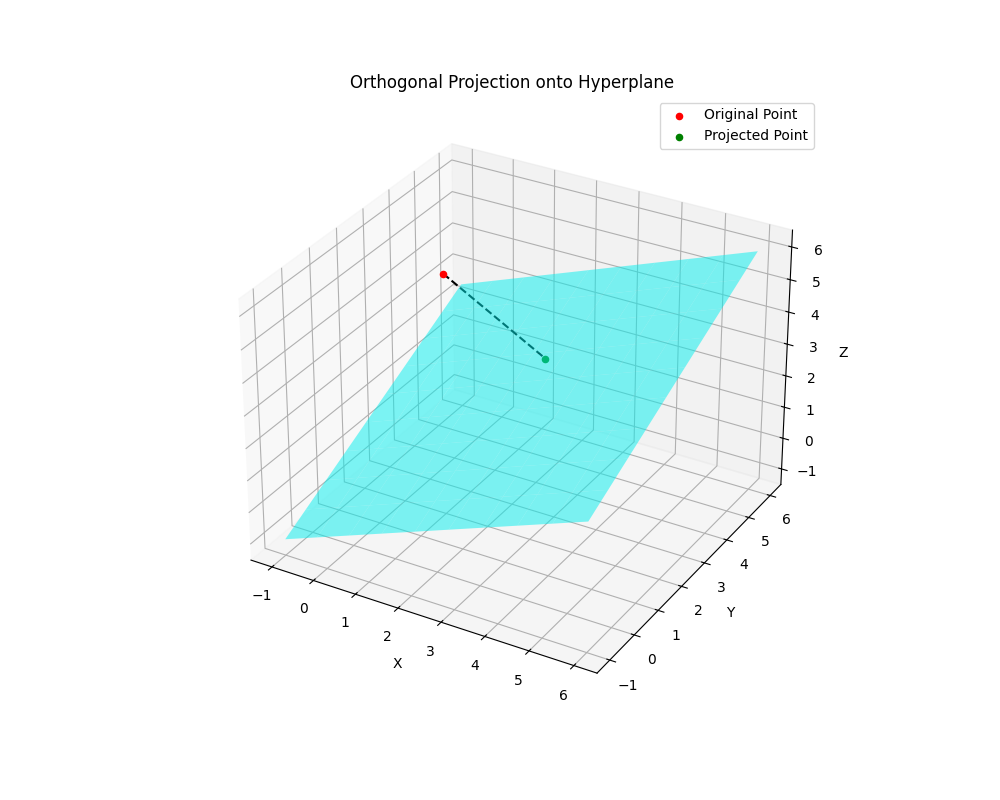
\includegraphics[width=0.6\linewidth]{../illustrations/orthogonal_projection.png}
   \caption{$QQ^{T}$ projects vector $v$ to the hyperplane generated by the column vector of $Q$, i.e. $q_{1}=[1/\sqrt{3}, 1\sqrt{3}, 1\sqrt{3}]$ and $q_{2}=[1/\sqrt{2}, -1/\sqrt{2}, 0]$. For instance, point $[1\; 2\; 6]^{T}$ in red is projected to $[1.5\quad 2.5\quad 3]^{T}$}
   \label{fig:enter-label2}
\end{figure}


We need prepare some lemmas to be at bottom of simultaneous iteration, assume $V$ is matrix consisting of linearly independent columns $[v_{1}, v_{2}, \cdots, v_{k}]$ and we have the following proposition
\begin{Lemma}
\begin{enumerate}
   \item $V$ is injective is equivalent to $\widehat{V}$ is injective.
   
   \item $PV$ is injective is equivalent to $\widehat{P}\widehat{V}$ is injective.
   
   \item $PV$ is injective implies that $V$ is injective.
\end{enumerate}
   
\end{Lemma}

\begin{proof}
   The first can be easily proven by $v_{i} = Q Q^{*} v_{i} = Q\widehat{v}_{i}$. 

   We can view $PV$ as new matrix consisting of $w_{i}$ and find that $\widehat{PV} = \widehat{P} \widehat{V}$.
\end{proof}


\end{document}